% 导入配置
% \documentclass[lang = cn, scheme = chinese, thmcnt = section]{elegantbook}
% elegantbook      设置elegantbook文档类
% lang = cn        设置中文环境
% scheme = chinese 设置标题为中文
% thmcnt = section 设置计数器


%% 1.封面设置

\title{Algebra Chapter 0 - Paolo Aluffi - NoteBook}                % 文档标题

\author{若水}               % 作者

\myemail{ethanmxzhou@163.com} % 邮箱

\homepage{helloethanzhou.github.io} % 主页

\date{\today}               % 日期

\extrainfo{上善若水任方圆}   % 箴言

\logo{PiCreatures_happy.pdf}        % 设置Logo

\cover{阿基米德螺旋曲线.pdf}          % 设置封面图片

% 修改标题页的色带
\definecolor{customcolor}{RGB}{135, 206, 250} 
% 定义一个名为customcolor的颜色,RGB颜色值为(135, 206, 250)

\colorlet{coverlinecolor}{customcolor}     % 将coverlinecolor颜色设置为customcolor颜色

%% 2.目录设置
\setcounter{tocdepth}{3}  % 目录深度为3

%% 3.引入宏包
\usepackage[all]{xy}
\usepackage{bbm, svg, graphicx, float, extpfeil, amsmath, amssymb, mathrsfs, mathalpha, boondox-cal, boondox-calo, hyperref, graphicx, romannum, chemarrow, booktabs, fontspec, ctex}

%% 4.定义命令
\newcommand{\N}{\mathbb{N}}            % 自然数集合
\newcommand{\R}{\mathbb{R}}            % 实数集合
\newcommand{\C}{\mathbb{C}}  		   % 复数集合
\newcommand{\Q}{\mathbb{Q}}            % 有理数集合
\newcommand{\Z}{\mathbb{Z}}            % 整数集合
\newcommand{\F}{\mathbb{F}}
\newcommand{\sub}{\subset}             % 包含
\newcommand{\im}{\text{im }}           % 像
\newcommand{\lang}{\langle}            % 左尖括号
\newcommand{\rang}{\rangle}            % 右尖括号
\newcommand{\dis}{\displaystyle}
\newcommand{\cont}{\text{cont}}
\newcommand{\cha}{\text{char}}
\newcommand{\function}[5]{
	\begin{align*}
		#1:\begin{aligned}[t]
			#2 &\longrightarrow #3\\
			#4 &\longmapsto #5
		\end{aligned}
	\end{align*}
}                                     % 函数

\newcommand{\lhdneq}{%
	\mathrel{\ooalign{$\lneq$\cr\raise.22ex\hbox{$\lhd$}\cr}}} % 真正规子群

\newcommand{\rhdneq}{%
	\mathrel{\ooalign{$\gneq$\cr\raise.22ex\hbox{$\rhd$}\cr}}} % 真正规子群

\newcommand{\upiff}{\mathrel{\rotatebox[origin=c]{90}{$\iff$}}} % 竖着的等价

\newcommand{\Rmnum}[1]{\uppercase\expandafter{\romannumeral #1}}  %定义命令输入大写罗马数字
\newcommand{\rmnum}[1]{\romannumeral #1}  %定义命令输入小写罗马数字



% \begin{document}
	
\chapter{环论$\rm\Rmnum{2}$}

\begin{figure}[H]
	\centering
	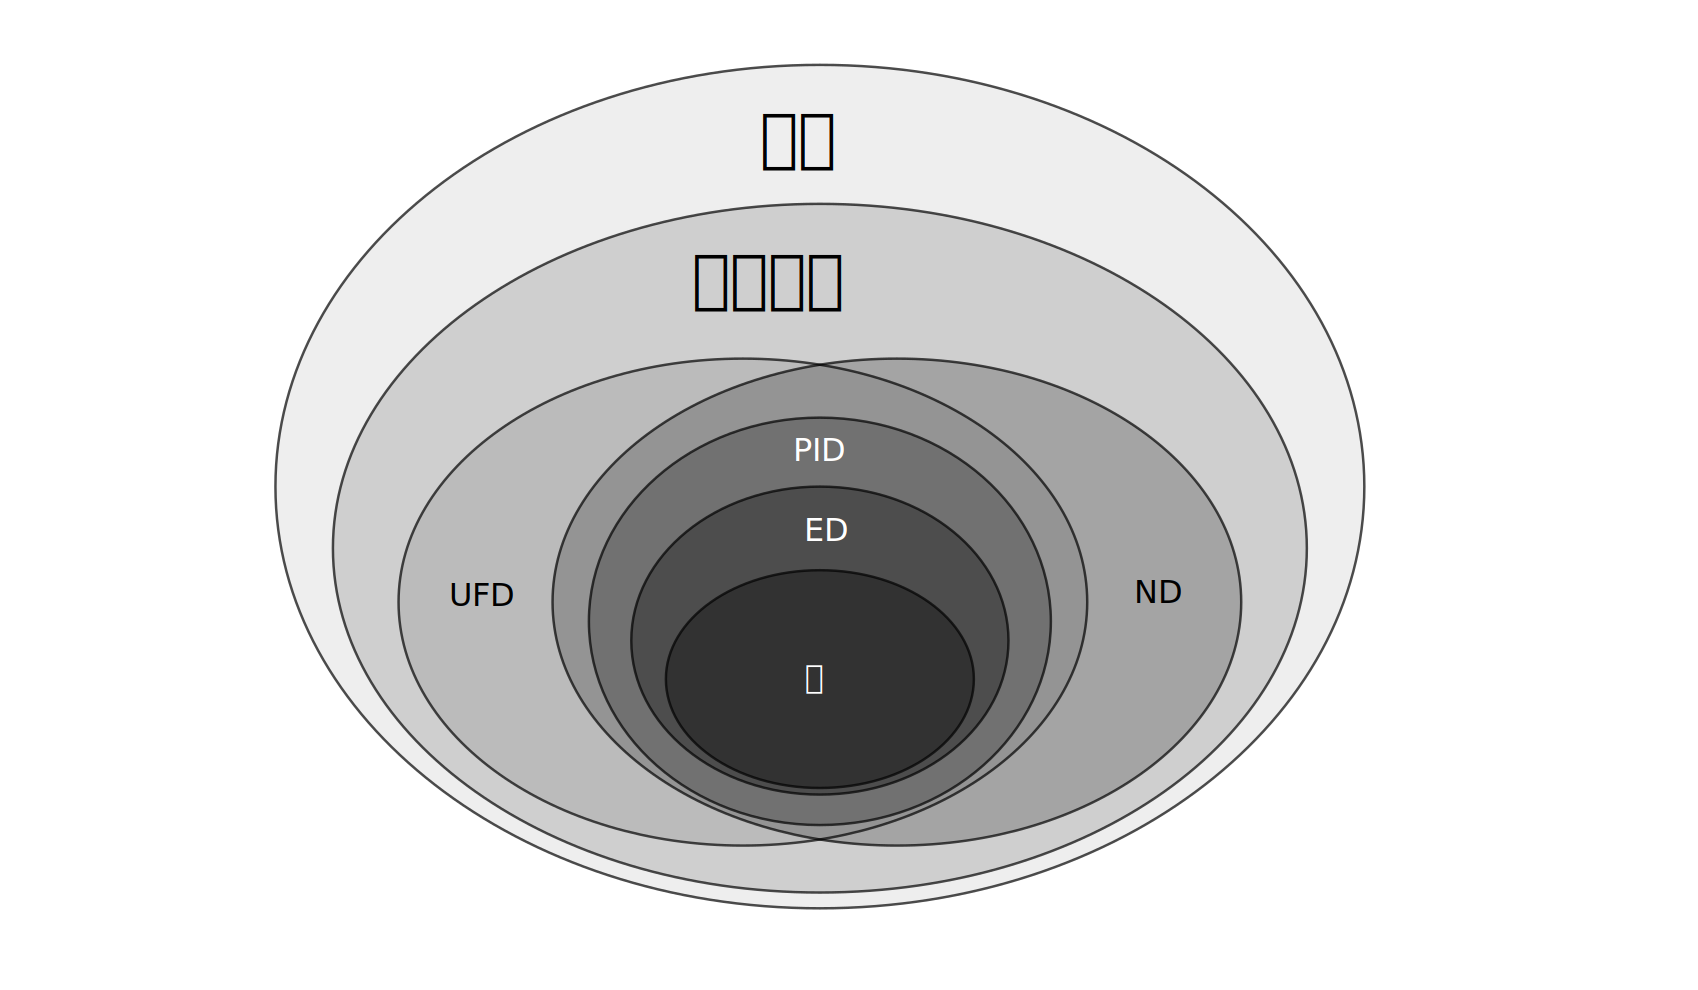
\includegraphics[scale = 0.5]{../figure/整环}
	\caption{整环的关系}
\end{figure}

\section{分解整环与Noether环}

\subsection{素元与不可约元}

\begin{definition}{整除 divide}
	对于交换环$(R,+,\;\cdot\;)$,称$a\in R$整除$b\in R$,并记作$a\mid b$,如果存在$c\in R$,使得成立$b=a\cdot c$。
\end{definition}

\begin{proposition}{整除的反身性与传递性}{整除的反身性与传递性}
	交换环元素间的整除关系具有反身性与传递性。
\end{proposition}

\begin{proof}
	对于反身性,显然$a=a\cdot 1$,因此$a\mid a$。
	
	对于传递性,如果$a\mid b$,且$b\mid c$,那么存在$u,v\in R$,使得成立$b=a\cdot u$,且$c=b\cdot v$,那么$c=(u\cdot v)\cdot a$,因此$a\mid c$。
\end{proof}

\begin{lemma}{整除的等价条件}{整除的等价条件}
	对于整环$(R,+,\;\cdot\;)$的非零元$a,b\in R$,成立
	$$
	a\mid b
	\iff b\in (a)
	\iff (b)\sub (a)
	$$
\end{lemma}

\begin{proof}
	如果$(b)\sub (a)$,那么显然$b\in (a)$。
	
	如果$b\in (a)$,那么存在$c\in R$,使得成立$b=a\cdot c$,因此$a\mid b$。
	
	如果$a\mid b$,那么存在$c\in R$,使得成立$b=a\cdot c$。任取$x\in (b)$,存在$d\in R$,使得成立$x=b\cdot d$,因此
	$$
	x=b\cdot d=(c\cdot d)\cdot a\in (a)
	$$
	由$x$的任意性,$(b)\sub (a)$。
\end{proof}

\begin{definition}{因子 divisor}
	对于交换环$(R,+,\;\cdot\;)$,称$a\in R$为$b\in R$的因子,如果成立$a\mid b$。
\end{definition}

\begin{definition}{倍元 multiple}
	对于交换环$(R,+,\;\cdot\;)$,称$b\in R$为$a\in R$的倍元,如果成立$a\mid b$。
\end{definition}

\begin{definition}{相伴元 associate element}
	对于交换环$(R,+,\;\cdot\;)$,称$a\in R$与$b\in R$相伴,并记作$a\sim b$,如果成立$a\mid b$,且$b\mid a$。
\end{definition}

\begin{proposition}{相伴为等价条件}{相伴为等价条件}
	交换环元素间的相伴关系为等价关系。
\end{proposition}

\begin{proof}
	对于自反性,显然$a\mid a$,因此$a\sim a$。
	
	对于对称性,如果$a\sim b$,那么$a\mid b$,且$b\mid a$,因此$b\sim a$。
	
	对于传递性,如果$a\sim b$,且$b\sim c$,那么
	$$
	a\mid b,\qquad 
	b\mid a,\qquad 
	b\mid c,\qquad 
	c\mid b
	$$
	由整除关系的传递性\ref{pro:整除的反身性与传递性},$a\mid c$,且$c\mid a$,那么$a\sim c$。
\end{proof}

\begin{lemma}{相伴的等价条件}{相伴的等价条件}
	对于整环$(R,+,\;\cdot\;)$的非零元$a,b\in R$,成立
	$$
	a\mid b\text{ 且 }b\mid a
	\iff (a)=(b)
	\iff 
	\exists\text{ 单位 }u\in R,a=u\cdot b
	$$
\end{lemma}

\begin{proof}
	由引理\ref{lem:整除的等价条件},成立
	$$
	a\mid b\text{ 且 }b\mid a
	\iff (a)=(b)
	$$
	下面证明
	$$
	a\mid b\text{ 且 }b\mid a
	\iff 
	\exists\text{ 单位 }u\in R,a=u\cdot b
	$$
	
	对于必要性,如果$a\mid b$,且$b\mid a$,那么存在$c,d\in R$,使得成立$a=b\cdot c$,且$b=a \cdot d$,那么
	$$
	a=b\cdot c=c\cdot d\cdot a\implies (c \cdot d-1)a=0
	$$
	由消去律,$c\cdot d=1$,因此$c$为单位。
	
	对于充分性,如果存在单位$u\in R$,使得成立$a=u\cdot b$,那么$b\mid a$,且存在$v\in R$,使得成立$v\cdot u=1$,因此
	$$
	b=1\cdot b=v\cdot u \cdot b=v \cdot a
	$$
	于是$b\mid a$。
\end{proof}

\begin{definition}{素元 prime element}
	对于整环$(R,+,\;\cdot\;)$,称$p\in R$为素元,如果$p$不为零元,且$p$不为单位,同时成立如下命题之一。
	\begin{enumerate}
		\item $p\mid a\cdot b\implies p\mid a$或$p\mid b$
		\item $(p)$为$R$的素理想。
	\end{enumerate}
\end{definition}

\begin{definition}{可约元 reducible element}
	对于整环$(R,+,\;\cdot\;)$,称$p\in R$为可约元,如果$p$或为零元,或为单位,或成立如下命题之一。
	\begin{enumerate}
		\item 存在非单位的元素$a,b\in R$,使得成立$p = a \cdot b$。
		\item 存在非相伴的元素$a,b\in R$,使得成立$p = a \cdot b$。
		\item 存在$a,b\in R$,使得成立$p = a \cdot b$,同时$(p)\subsetneq (a)$,且$(p)\subsetneq (b)$。
		\item 存在$q\in R$,使得成立$(p)\subsetneq (q) \subsetneq (1)$。
	\end{enumerate}
\end{definition}

\begin{definition}{不可约元 irreducible element}
	对于整环$(R,+,\;\cdot\;)$,称$p\in R$为不可约元,如果$p$不为零元,且$p$不为单位,同时成立如下命题之一。
	\begin{enumerate}
		\item $p = a \cdot b \implies a$为单位或$b$为单位。
		\item $p = a\cdot b\implies p$与$a$相伴或$p$与$b$相伴。
		\item $p = a\cdot b\implies (p)=(a)$或$(p)=(b)$。
		\item $(p)\sub (q)\implies (p)=(q)$或$(q)=(1)$。
	\end{enumerate}
\end{definition}

\begin{lemma}{素元不可约}{素元不可约}
	对于整环$(R,+,\;\cdot\;)$,如果$p\in R$为素元,那么$p$为不可约元。
\end{lemma}

\begin{proof}
	任取$a,b\in R$,使得成立$p=a\cdot b$,因此$a\cdot b\in (p)$。一方面,由于$p$为素元,那么$(p)$为非零素理想,因此$a\in (p)$,或$b\in (p)$。不妨$a\in (p)$,那么$(a)\sub (p)$。另一方面,由于$p=a\cdot b\in (a)$,那么$(p)\sub (a)$。综合两方面,$(p)=(a)$,进而$p$为不可约元。
\end{proof}

\subsection{分解整环}

\begin{definition}{完全因子分解 factorization into irreducibles}
	对于整环$(R,+,\;\cdot\;)$,称$r\in R$可完全因子分解,如果存在不可约元$p_1,\cdots,p_n\in R$,使得成立
	$$
	r=p_1\cdots p_n
	$$
\end{definition}

\begin{definition}{唯一完全因子分解 unique factorization into irreducibles}
	对于整环$(R,+,\;\cdot\;)$,称$r\in R$可唯一完全因子分解,如果存在不可约元$p_1,\cdots,p_n\in R$,使得成立
	$$
	r=p_1\cdots p_n
	$$
	且若不可约元$q_1,\cdots,q_m\in R$成立
	$$
	r=q_1\cdots q_m
	$$
	则$m=n$,且存在双射$\tau:\N^*\to\N^*$,使得对于任意$1\le k\le n$,$p_k$与$q_{\tau(k)}$相伴。
\end{definition}

\begin{definition}{分解整环 domains with factorizations}
	称整环为分解整环,如果其任意非零非单位的元素可完全因子分解。
\end{definition}

\begin{definition}{唯一因子分解整环 unique factorization domain, UFD}
	称整环为唯一因子分解整环,如果其任意非零非单位的元素可唯一完全因子分解。
\end{definition}

\begin{lemma}{整除的等价条件}{整除的等价条件2}
	对于UFD $(R,+,\;\cdot\;)$的非零元$a,b\in R$,并记$a$的不可约因子族构成多重集合$A$,$b$的不可约因子族构成多重集合$B$,成立
	$$
	a\mid b
	\iff b\in (a)
	\iff (b)\sub (a)
	\iff A\le B
	$$
\end{lemma}

\begin{proof}
	由引理\ref{lem:整除的等价条件},成立
	$$
	a\mid b
	\iff b\in (a)
	\iff (b)\sub (a)
	$$
	
	如果$a\mid b$,那么存在$c\in R$,使得成立$b=a\cdot c$。由于$R$为UFD,那么记$a$与$c$的唯一完全因子分解为
	$$
	a=p_1\cdots p_n,\qquad 
	c=q_1\cdots q_m
	$$
	因此
	$$
	b=p_1\cdots p_nq_1\cdots q_m
	$$
	那么
	$$
	A=\{ p_1,\cdots ,p_n \},\qquad 
	B=\{ p_1,\cdots ,p_n ,q_1,\cdots ,q_m \}
	$$
	进而$A\le B$。
	
	如果$A\le B$,那么由$R$为UFD,记$a$与$b$的唯一完全因子分解为
	$$
	a=p_1^{i_1}\cdots p_n^{i_n},\qquad 
	b=p_1^{j_1}\cdots p_n^{j_n}q_1^{k_1}\cdots q_m^{k_m}
	$$
	其中$p_1,\cdots,p_n,q_1,\cdots,q_m$为不可约元,且
	$$
	i_1,\cdots,i_n,j_1,\cdots,j_n,k_1,\cdots,k_m\in\N^*
	$$
	由于$A\le B$,那么
	$$
	i_1\le j_1\qquad \cdots\qquad i_n\le j_n
	$$
	记
	$$
	c=p_1^{j_1-i_1}\cdots p_n^{j_n-i_n}q_1^{k_1}\cdots q_m^{k_m}
	$$
	因此$b=a\cdot c$,进而$a\mid b$。
\end{proof}

\begin{lemma}{相伴的等价条件}{相伴的等价条件2}
	对于UFD $(R,+,\;\cdot\;)$的非零元$a,b\in R$,并记$a$的不可约因子族构成多重集合$A$,$b$的不可约因子族构成多重集合$B$,成立
	$$
	a\mid b\text{ 且 }b\mid a
	\iff (a)=(b)
	\iff 
	\exists\text{ 单位 }u\in R,a=u\cdot b
	\iff A=B
	$$
\end{lemma}

\begin{proof}
	由引理\ref{lem:整除的等价条件2}与\ref{lem:相伴的等价条件},命题显然。
\end{proof}

\subsection{Noether环}

\begin{definition}{稳定的 stabilize}
	对于偏序集$(S,\preceq)$,称增序列
	$$
	s_1\preceq s_2\preceq s_3\preceq\cdots
	$$
	为稳定的,如果存在$N\in\N^*$,使得对于任意$n\ge N$,成立$s_n=s_N$。
\end{definition}

\begin{definition}{升链条件 ascending chain condition, a.c.c.}
	称偏序集$(S,\preceq)$成立升链条件,如果其任意增序列稳定。
\end{definition}

\begin{definition}{极大条件 maximal element condition}
	称偏序集$(S,\preceq)$成立极大条件,如果其任意非空子集存在极大元。
\end{definition}

\begin{theorem}{升链条件$\iff$极大条件}{升链条件与极大条件等价}
	对于偏序集,成立
	$$
	\text{升链条件}\iff \text{极大条件}
	$$
\end{theorem}

\begin{proof}
	如果偏序集$(S,\preceq)$成立极大条件,即其任意非空子集存在极大元,那么对于任意增序列
	$$
	s_1\preceq s_2\preceq s_3\preceq\cdots
	$$
	构成的非空子集$\{s_n\}_{n=1}^{\infty}$存在极大元$x_N$,因此对于任意$n\ge N$,成立$s_n=s_N$,那么该增序列稳定,进而该偏序集$(S,\preceq)$成立升链条件。
	
	如果偏序集$(S,\preceq)$不成立极大条件,即存在非空子集$T\sub S$,使得对于任意$x\in T$,存在$y\in T$,使得成立$x\ne y$,且$x\preceq y$,那么由数学归纳法,存在增序列$\{ s_n \}_{n=1}^{\infty}$,使得对于任意$n\in\N^*$,成立$s_{n}\ne s_{n+1}$,进而该偏序集$(S,\preceq)$不成立升链条件。
\end{proof}

\begin{definition}{Noether环}
	称交换环$(R,+,\;\cdot\;)$为Noether环,如果成立如下命题之一。
	\begin{enumerate}
		\item $R$的任意理想为有限生成理想。
		\item $R$成立理想升链条件。
		\item $R$成立理想极大条件。
	\end{enumerate}
\end{definition}

\begin{proof}
	由定理\ref{thm:升链条件与极大条件等价},成立
	$$
	R\text{ 成立理想升链条件}\iff
	R\text{ 成立理想极大条件}
	$$
	下面证明
	$$
	R\text{ 的任意理想为有限生成理想}\iff
	R\text{ 成立理想升链条件}
	$$
	
	如果$R$的任意理想为有限生成理想,但是$R$不成立理想升链条件,那么存在无限理想序列
	$$
	I_1\subsetneq I_2 \subsetneq I_3 \subsetneq \cdots
	$$
	记$\displaystyle I=\bigcup_{n=1}^{\infty}I_n$,那么$I$为$R$的理想。由于$R$的任意理想为有限生成理想,那么存在$\{r_k\}_{k=1}^{n}$,使得成立$I=(r_k)_{k=1}^{n}$,因此对于任意$1\le k\le n$,存在$n_k\in\N^*$,使得成立$r_k\in I_{n_k}$。记$\displaystyle N=\max_{1\le k\le n}n_k$,那么对于任意$1\le k\le n$,成立$r_k\in I_N$,进而$\displaystyle I\sub I_N=\bigcup_{n=1}^{N}I_n$。而$\displaystyle \bigcup_{n=1}^{N}I_n\sub I$,因此$\displaystyle I=\bigcup_{n=1}^{N}I_n$,产生矛盾!
	
	如果$R$成立理想升链条件,但是存在无限生成理想$I$,那么由数学归纳法,存在$\{ r_n \}_{n=1}^{\infty}\sub I$,使得无限理想序列
	$$
	(r_1)\subsetneq (r_1,r_2)\subsetneq (r_1,r_2,r_3) \subsetneq \cdots
	$$
	产生矛盾!
\end{proof}

\begin{proposition}{Noether环的像为Noether环}{Noether环的像为Noether环}
	对于环同态映射$\varphi:R\to S$,如果$(R,+,\;\cdot\;)$为Noether环,那么$\im \varphi$为Noether环。
\end{proposition}

\begin{proof}
	任取$\im \varphi$的理想$J$,由命题\ref{pro:理想的原像为理想},$\varphi^{-1}(J)$为$R$的理想。由于$R$为Noether环,那么存在$\{ r_k \}_{k=1}^{n}\sub R$,使得成立$\varphi^{-1}(J)=(r_k)_{k=1}^{n}$,进而$J=(\varphi(r_k))_{k=1}^{n}$,从而$\im \varphi$为Noether环。
\end{proof}

\begin{theorem}{ND$\implies$分解整环}
	Noether环为分解整环。
\end{theorem}

\begin{proof}
	对于$(R,+,\;\cdot\;)$,任取非零非单位的元素$r\in R$。如果$r$为不可约元,那么$r$可完全因子分解。
	
	如果$r$为可约元,那么存在$r_1,s_1\in R$,使得成立$r=r_1\cdot s_1$,同时$(r)\subsetneq (r_1)$,且$(r)\subsetneq (s_1)$。若$r_1$与$s_1$为不可约元,那么$r$可完全因子分解。若$r_1$为可约元,则重复如上过程。如果对于每一次过程,$r_n$均可约,那么可得无限理想序列
	$$
	(r)\subsetneq (r_1)\subsetneq (r_2) \subsetneq \cdots
	$$
	与$R$为Noether环矛盾!
	
	综上所述,$r$可完全因子分解,进而$R$为分解整环。
\end{proof}

\begin{theorem}{PID$\implies$ND}{PID为ND}
	PID为Noether环。
\end{theorem}

\begin{proof}
	任取PID $(R,+,\;\cdot\;)$的递增主理想序列
	$$
	I_1\sub I_2\sub \cdots \sub I_n\sub \cdots 
	$$
	由于$R$为PID,那么存在$\{a_n\}_{n=1}^{\infty}\sub R$,使得对于任意$n\in\N^*$,成立$I_n=(a_n)$。定义
	$$
	I=\bigcup_{n=1}^{\infty}I_n=\bigcup_{n=1}^{\infty}(a_n)
	$$
	那么$I$为$R$的理想,因此存在$a\in R$,使得成立$I=(a)$。由于$a\in \bigcup(a_n)$,那么存在$N\in\N^*$,使得成立$a\in (a_N)$,进而$(a)\sub (a_N)$。又因为$(a_N)\sub (a)$,那么$(a)=(a_N)$,因此对于任意$n\ge N$,成立$(a_n)=(a_N)$,进而$R$成立理想升链条件,于是$R$为Noether环。
\end{proof}

\begin{theorem}
	对于Noether环$(R,+,\;\cdot\;)$,如果$I$为多项式环$R[x_1,\cdots,x_n]$的理想,那么商环$R[x_1,\cdots,x_n]/I$为Noether环。
\end{theorem}

\begin{lemma}{Hilbert基定理}{Hilbert基定理}
	$$
	R\text{ 为Noether环}\iff
	R[x]\text{ 为Noether环}
	$$
\end{lemma}

\begin{definition}{Noether模}
	对于交换环$(R,+,\;\cdot\;)$,称$R$-模$M$为Noether模,如果成立如下命题之一。
	\begin{enumerate}
		\item $M$的任意子模为有限生成的。
		\item $M$的任意升子模链有限。
		\item $M$的任意子模族存在极大子模。
	\end{enumerate}
\end{definition}

\section{UFD,PID,ED}

\subsection{最大公因子}

\begin{definition}{公因子 common divisor}
	对于整环$(R,+,\;\cdot\;)$,称$d\in R$为$a,b\in R$的公因子,如果成立如下命题之一。
	\begin{enumerate}
		\item $(a,b)\sub (d)$
		\item $d\mid a$,且$d\mid b$。
	\end{enumerate}
\end{definition}

\begin{definition}{最大公因子 greatest common divisor}
	对于整环$(R,+,\;\cdot\;)$,称$a,b\in R$的公因子$d\in R$为最大公因子,如果成立如下命题之一。
	\begin{enumerate}
		\item $(a,b)=(d)$
		\item 对于任意$a,b$的公因子$d'$,成立$d'\mid d$。
	\end{enumerate}
\end{definition}

\begin{definition}{最大公因子条件 greatest common divisor condition}
	称整环$(R,+,\;\cdot\;)$成立最大公因子条件,如果其任意非零元间存在最大公因子。
\end{definition}

\begin{lemma}{UFD$\implies$最大公因子条件}{UFD成立最大公因子条件}
	UFD成立最大公因子条件。
\end{lemma}

\begin{proof}
	对于UFD $(R,+,\;\cdot\;)$,任取非零元$a,b\in R$,作唯一完全因子分解
	$$
	a=u\cdot p_1^{\alpha_1}\cdots p_n^{\alpha_n},\qquad 
	b=v\cdot p_1^{\beta_1}\cdots p_n^{\beta_n}
	$$
	其中$u,v$为单位,且对于任意$1\le k\le n$,成立$\alpha_k,\beta_n\in\N$。记
	$$
	d=p_1^{\min(\alpha_1,\beta_1)}\cdots p_n^{\min(\alpha_n,\beta_n)}
	$$
	由于
	$$
	a=u\cdot p_1^{\alpha_1-\min(\alpha_1,\beta_1)}\cdots p_n^{\alpha_n-\min(\alpha_n,\beta_n)}\cdot d,\qquad 
	b=v\cdot p_1^{\beta_1-\min(\alpha_1,\beta_1)}\cdots p_n^{\beta_n-\min(\alpha_n,\beta_n)}\cdot d
	$$
	那么$a\mid d$且$b\mid d$,因此$d$为$a,b$的公因子。任取$a,b$的公因子$c$,由引理\ref{lem:整除的等价条件2},作唯一完全因子分解
	$$
	c=w\cdot p_1^{\gamma_1}\cdots p_n^{\gamma_n}
	$$
	其中对于任意$1\le k\le n$,成立$\gamma_k\ge \min(\alpha_k,\beta_k)$。由于
	$$
	c=w\cdot p_1^{\gamma_1-\min(\alpha_1,\beta_1)}\cdots p_n^{\gamma_n-\min(\alpha_1,\beta_1)}\cdot d
	$$
	那么$c\mid d$,进而$d$为$a,b$的最大公因子。
\end{proof}

\subsection{UFD}

\begin{definition}{素元性条件 prime element condition}{素元性条件}
	称整环$(R,+,\;\cdot\;)$成立素元性条件,如果对于其任意不可约元为素元。
\end{definition}

\begin{lemma}{}{最大公因子条件推出素元性条件引理}
	如果整环$(R,+,\;\cdot\;)$成立最大公因子条件,那么对于任意$a,b,c\in R$,成立$\mathrm{gcd}(a\cdot b,a\cdot c)\sim a\cdot \mathrm{gcd}(b,c)$
\end{lemma}

\begin{proof}
	如果$a=0$,那么$\mathrm{gcd}(a\cdot b,a\cdot c)\sim a\cdot \mathrm{gcd}(b,c)\sim 0$。
	
	如果$\mathrm{gcd}(b,c)=0$,那么$b=c=0$,从而$\mathrm{gcd}(a\cdot b,a\cdot c)\sim a\cdot \mathrm{gcd}(b,c)\sim 0$。
	
	如果$a\ne 0$且$\mathrm{gcd}(b,c)\ne 0$,由于$\mathrm{gcd}(b,c)\mid b$且$\mathrm{gcd}(b,c)\mid c$,那么$a\cdot \mathrm{gcd}(b,c)\mid a\cdot b$且$a\cdot \mathrm{gcd}(b,c)\mid a\cdot c$,进而$a\cdot \mathrm{gcd}(b,c)\mid \mathrm{gcd}(a\cdot b,a\cdot c)$,因此存在$u\in R$,使得成立$\mathrm{gcd}(a\cdot b,a\cdot c)=a\cdot u\cdot \mathrm{gcd}(b,c)$。由于$\mathrm{gcd}(a\cdot b,a\cdot c)\mid a\cdot b$,那么存在$v\in R$,使得成立$a\cdot b=v\cdot \mathrm{gcd}(a\cdot b,a\cdot c)$,因此$a\cdot b=v\cdot a\cdot u\cdot \mathrm{gcd}(b,c)$。由消去律,$b=v\cdot u\cdot \mathrm{gcd}(b,c)$,进而$u\cdot \mathrm{gcd}(b,c)\mid b$。同理,$u\cdot \mathrm{gcd}(b,c)\mid c$,进而$u\cdot \mathrm{gcd}(b,c)\mid \mathrm{gcd}(b,c)$,因此存在$u'\in R$,使得成立$\mathrm{gcd}(b,c)=u\cdot u'\cdot \mathrm{gcd}(b,c)$,由消去律$u\cdot u'=1$,进而$u$为单位,那么$\mathrm{gcd}(a\cdot b,a\cdot c)\sim a\cdot \mathrm{gcd}(b,c)$。
\end{proof}

\begin{lemma}{最大公因子条件$\implies$素元性条件}{最大公因子条件推出素元性条件}
	如果整环$(R,+,\;\cdot\;)$成立最大公因子条件,那么$R$成立素元性条件。
\end{lemma}

\begin{proof}
	任取不可约元$p\in R$,取$a,b\in R$使得成立$p\mid a\cdot b$。由于$\mathrm{gcd}(p,a)\mid p$,那么或$\mathrm{gcd}(p,a)\sim p$,或$\mathrm{gcd}(p,a)$为单位。
	
	如果$\mathrm{gcd}(p,a)\sim p$,那么$p\mid \mathrm{gcd}(p,a)$,因此$p\mid a$。
	
	如果$\mathrm{gcd}(p,a)$为单位,那么$\mathrm{gcd}(p,a)\sim 1$,因此$b\cdot \mathrm{gcd}(p,a)\sim b$。由引理\ref{lem:最大公因子条件推出素元性条件引理},$\mathrm{gcd}(p\cdot b,a\cdot b)\sim b$。由于$p\mid p\cdot b$,且$p\mid a\cdot b$,那么$p\mid \mathrm{gcd}(p\cdot b,a\cdot b)$,进而$p\mid b$。
	
	综上所述,$p$为素元,进而$R$成立素元性条件。
\end{proof}

\begin{lemma}{UFD$\implies$素元性条件}{UFD成立素元性条件}
	UFD成立素元性条件。
\end{lemma}

\begin{proof}
	(法一)由引理\ref{lem:UFD成立最大公因子条件}与\ref{lem:最大公因子条件推出素元性条件},命题得证!
	
	(法二)对于UFD $(R,+,\;\cdot\;)$,任取不可约元$p\in R$,取$a,b\in R$使得成立$p\mid a\cdot b$。分别记$p,a,b$的不可约因子族构成的多重集合为$P,A,B$,那么由引理\ref{lem:整除的等价条件2}
	$$
	P=\{p\}\le A\sqcup B
	$$
	那么不妨$P\le A$,因此由引理\ref{lem:整除的等价条件2},$p\mid a$,进而$p$为素元。
\end{proof}

\begin{definition}{主理想升链条件 ascending chain condition for principal ideal}
	称整环$(R,+,\;\cdot\;)$成立主理想升链条件,如果其任意递增主理想序列稳定。
\end{definition}

\begin{lemma}{UFD$\implies$主理想升链条件}{UFD成立主理想升链条件}
	UFD成立主理想升链条件。
\end{lemma}

\begin{proof}
	对于对于UFD $(R,+,\;\cdot\;)$,任取严格递增主理想序列
	$$
	(a_1)\subsetneq (a_2)\subsetneq \cdots \subsetneq (a_n)\subsetneq \cdots 
	$$
	那么由引理\ref{lem:整除的等价条件}与\ref{lem:相伴的等价条件},对于任意$n\in\N^*$,$a_{n+1}$为$a_n$的非相伴因子。
	
	如果$a_1=0$,那么对于任意$n\in\N^*$,$a_n=0$。
	
	如果$a_1$为单位,那么对于任意$n\in\N^*$,$(a_n)=(1)$。
	
	如果$a_1$非零且非单位,那么对于$a_1$作唯一完全因子分解
	$$
	a_1=p_1\cdots p_n
	$$
	其中$p_1,\cdots,p_n$为不可约元,显然$a_1$的非相伴因子有限。
	
	综上所述,$R$成立主理想升链条件。
\end{proof}

\begin{lemma}{素元性条件+主理想升链条件$\implies$UFD}{素元性条件+主理想升链条件推出UFD}
	如果整环$(R,+,\;\cdot\;)$成立素元性条件与主理想升链条件,那么$R$为UFD。
\end{lemma}

\begin{proof}
	对于存在性,任取非零非单位的元素$a\in R$,如果$a$为不可约元,那么$a$可完全因子分解。如果$a$为可约元,那么由主理想升链条件,$a$存在不可约因子$p_1$,于是$a=p_1a_1$。如果$a_1$不可约,那么$a$可完全因子分解。如果$a_1$可约,那么重复上述过程,结合主理想升链条件,可得$a$的完全因子分解$a=p_1\cdots p_n$。
	
	对于唯一性,如果非零非单位的元素$a\in R$存在完全因子分解
	$$
	a=p_1\cdots p_n=q_1\cdots q_m
	$$
	对于$n$进行归纳。当$n=1$时
	$$
	a=p_1=q_1\cdots q_m
	$$
	如果$m\ge 2$,那么
	$$
	p_1=q_1(q_2\cdots q_m)
	$$
	由于$p_1$不可约,那么$p_1$与$q_1$相伴,进而存在单位$u\in R$,使得成立$q_1=p_1u$,因此$p_1=p_1u(q_2\cdots q_m)$。由消去律,$1=u(q_2\cdots q_m)$,进而$q_2$为单位,矛盾!从而$m=1$,命题得证!
	
	假设当$n=k$时,命题成立,那么当$n=k+1$时,由于$p_1$不可约,那么由素元性条件,$p_1$为素元。由于$p_1\mid q_1\cdots q_m$,那么不妨$p_1\mid q_1$。由于$q_1$不可约,那么$p_1\sim q_1$,进而存在单位$v\in R$,使得成立$p_1=q_1v$,进而
	$$
	q_1vp_2\cdots p_{k+1}=q_1\cdots q_m
	$$
	由消去律
	$$
	vp_2\cdots p_{k+1}=q_2\cdots q_m
	$$
	由归纳假设,$n=k+1$时命题得证!
	
	综上所述,$R$为UFD。
\end{proof}

\begin{theorem}{UFD的等价条件}
	对于整环$(R,+,\;\cdot\;)$,成立
	$$
	R \text{ 为UFD}
	\iff
	R \text{ 成立最大公因子条件、素元性条件与主理想升链条件}
	$$
\end{theorem}

\begin{proof}
	由引理\ref{lem:UFD成立最大公因子条件}、\ref{lem:最大公因子条件推出素元性条件}、\ref{lem:UFD成立素元性条件}、\ref{lem:UFD成立主理想升链条件}、\ref{lem:素元性条件+主理想升链条件推出UFD},命题得证!
\end{proof}

\subsection{PID$\implies$UFD}

\begin{theorem}{PID$\implies$UFD}{PID为UFD}
	PID为UFD。
\end{theorem}

\begin{proof}
	对于PID $(R,+,\;\cdot\;)$,任取不可约元$p$,由命题\ref{pro:PID的非零素理想为极大理想},$(p)$为非零极大理想,进而为非零素理想,因此$p$为素元,从而$R$成立素元性条件。
	
	由定理\ref{thm:PID为ND},$R$成立理想升链条件。特别的,$R$成立主理想升链条件。
	
	由引理\ref{lem:素元性条件+主理想升链条件推出UFD},$R$为UFD。
\end{proof}

\subsection{Euclid整环}

\begin{definition}{Euclid整环}
	称整环$(R,+,\;\cdot\;)$为Euclid整环,如果存在映射$v:R\setminus\{0\}\to \N$,使得对于任意$a\in R$与$b\in R\setminus\{0\}$,存在$q,r\in R$,使得成立
	$$
	a=q\cdot b+r,\qquad 
	r=0\text{ 或 }r\ne 0,v(r)<v(b)
	$$
\end{definition}

\begin{theorem}{ED$\implies$PID}{ED为PID}
	ED为PID。
\end{theorem}

\begin{proof}
	对于Euclid整环$(R,+,\;\cdot\;)$,任取非零理想$I$,令$b\in I\setminus\{0\}$满足对于任意$r\in I\setminus\{0\}$,成立$v(b)\le v(x)$,那么$(b)\sub I$。任取$a\in I$,由于$R$为Euclid整环,那么存在$q,r\in R$,使得成立
	$$
	a=q\cdot b+r,\qquad 
	r=0\text{ 或 }r\ne 0,v(r)<v(b)
	$$
	
	如果$r\ne 0$,那么与$b$的定义矛盾!因此$r=0$,于是$a=q\cdot b\in (b)$。由$a$的任意性,$I\sub (b)$,进而$I=(b)$。由$I$的任意性,$R$为PID。
\end{proof}

\begin{lemma}{}{Euclid算法引理}
	对于交换环$(R,+,\;\cdot \;)$,如果$a=q\cdot b+r$,那么$(a,b)=(b,r)$。
\end{lemma}

\begin{proof}
	由于$a=q\cdot b+r\in (b,r)$,那么$(a,b)\sub (b,r)$。由于$r=a-q\cdot b\in (a,b)$,那么$(a,b)\supset (b,r)$。进而$(a,b)=(b,r)$​。
\end{proof}

\begin{definition}{Euclid算法}
	对于Euclid整环$(R,+,\;\cdot \;)$,计算$a,b\in R$的最大公因子。使用带余除法
	\begin{align*}
		a & = b\cdot q_1 + r_1\\
		b & = r_1\cdot q_2 + r_2\\
		r_1 & = r_2\cdot q_3 + r_3\\
		& \cdots\\
		r_{n-2} & = r_{n-1}\cdot q_{n} + r_{n}\\
		r_{n-1} & = r_n\cdot q_{n+1}\\
	\end{align*}
	由引理\ref{lem:Euclid算法引理}
	$$
	(a,b)=
	(b,r_1)=
	(r_1,r_2)=
	\cdots=
	(r_{n-1},r_n)=(r_n)
	$$
	进而$\mathrm{gcd}(a,b)=r_n$。
\end{definition}

\section{间奏曲:Zorn引理}

\subsection{集合论:再一次邂逅}

\begin{definition}{序关系 ordered relation}
	称集合$S$上的关系$\preceq$为序关系,如果其成立如下性质。
	\begin{enumerate}
		\item 自反性(reflexivity):$a\preceq a$
		\item 反对称性(antisymmetry):$a\preceq b\text{ 且 }b\preceq a\implies a=b$
		\item 传递性(transitivity):$a\preceq b\text{ 且 }b\preceq c\implies a\preceq c$
	\end{enumerate}
\end{definition}

\begin{definition}{严格序关系 strict ordered relation}
	称集合$S$上的关系$\prec$为严格序关系,如果其成立如下性质。
	\begin{enumerate}
		\item 非自反性(irreflexivity):$\neg a\prec a$
		\item 非对称性(asymmetry):$a\prec b\implies \neg b\prec a$
		\item 传递性(transitivity):$a\prec b\text{ 且 }b\prec c\implies a\prec c$
	\end{enumerate}
\end{definition}

\begin{definition}{全序集 totally ordered set, toset / 链 chain}
	称集合结构$(S,\preceq)$为全序集,如果$\preceq$为$S$上的序关系,且对于任意$s,t\in S$,或成立$s\preceq t$,或成立$t\preceq s$。
\end{definition}

\begin{definition}{偏序集 partially ordered set, poset}
	称集合结构$(S,\preceq)$为偏序集,如果$\preceq$为$S$上的序关系,且存在子集$T\sub S$,使得$(T,\preceq)$为全序集。
\end{definition}

\begin{definition}{良序集 well ordered set, woset}
	称全序集$(S,\preceq)$为良序集,如果任意非空子集存在极小元。
\end{definition}

\begin{definition}{极大元 maximal element}
	对于偏序集$(S,\preceq)$,称$m\in S$为$S$的极大元,如果对于任意$s\in S$,成立
	$$
	m\preceq s\implies m=s
	$$
\end{definition}

\begin{definition}{极小元 least element}
	对于偏序集$(S,\preceq)$,称$\mathcal{s}\in S$为$S$的极小元,如果对于任意$s\in S$,成立
	$$
	s\preceq \mathcal{s}\implies s=\mathcal{s}
	$$
\end{definition}

\begin{definition}{上界 upper bound}
	对于偏序集$(S,\preceq)$,称$u\in S$为子集$T\sub S$的上界,如果对于任意$t\in T$,成立$t\preceq u$。
\end{definition}

\begin{theorem}{Zorn引理}{Zorn引理}
	对于偏序集$(S,\preceq)$,如果$S$的任意全序子集在$S$中存在上界,那么$S$存在极大元。
\end{theorem}

\begin{theorem}{选择公理 axiom of choice}{选择公理}
	如果$\mathscr{F}$为集合$S$的非空不交子集族,那么可以对于任意$X\in \mathscr{F}$,选择$x\in X$,使得被选择的所有元素构成集合。
\end{theorem}

\begin{theorem}{良序定理 well-ordering theorem}{良序定理}
	对于任意集合$S$,存在序关系$\preceq$,使得$(S,\preceq)$为良序集。
\end{theorem}

\begin{theorem}
	$$
	\text{Zorn引理}
	\iff
	\text{选择公理}
	\iff
	\text{良序定理}
	$$
\end{theorem}

\begin{theorem}{归纳原理 principle of induction}
	\begin{enumerate}
		\item 对于良序集$(S,\preceq)$,如果子集$T\sub S$成立
		$$
		\forall s\in S,\quad ((\forall t\in S,\quad (t\prec s\implies t\in T))\implies s\in T)
		$$
		那么$T=S$。
		\item 对于良序集$(S,\preceq)$,其极小元为$\mathcal{s}$,如果命题$P:S\to \text{Bool}$成立
		\begin{align*}
			& P(\mathcal{s})=\text{True}\\
			& \forall s\in S,\quad ((\forall t\in S,\quad (t\prec s\implies P(t)=\text{True}))\implies P(s)=\text{True})
		\end{align*}
		那么
		$$
		\forall s\in S,\quad P(s)=\text{True}
		$$
	\end{enumerate}
\end{theorem}

\begin{proof}
	事实上,$1\iff 2$。取
	\begin{align*}
		T=\{ s\in S:P(s)=\text{True} \}\iff
		\begin{aligned}
			P:\begin{aligned}[t]
				S & \longrightarrow \text{Bool}\\
				s & \longmapsto \begin{cases}
					\text{True},\quad s\in T\\
					\text{False},\quad s\notin T
				\end{cases}
			\end{aligned}
		\end{aligned}
	\end{align*}
	那么
	\begin{gather*}
		\forall s\in S,\quad ((\forall t\in S,\quad (t\prec s\implies t\in T))\implies s\in T)\\
		\upiff\\
		\forall s\in S,\quad ((\forall t\in S,\quad (t\prec s\implies P(t)=\text{True}))\implies P(s)=\text{True})
	\end{gather*}
	对于极小元$\mathcal{s}$,由于命题$\forall t\in S,(t\prec s\implies t\in T)$为False,那么$P(\mathcal{s})=\text{True}$。进而$1\iff 2$。
	
	下面证明原命题。如果$T\subsetneq S$,那么$S\setminus T\ne\varnothing$。由于$S$为良序集,那么$S\setminus T$存在极小元$\mathcal{s}^*\in S\setminus T$。由于对于任意$t\in S$,成立若$t\prec \mathcal{s}^*$,则$t\in T$,那么$\mathcal{s}^*\in T$,因此产生矛盾!进而原命题得证!
\end{proof}

\subsection{应用:极大理想的存在性}

\begin{theorem}{极大理想的存在性}{极大理想的存在性}
	对于交换环$(R,+,\;\cdot \;)$,如果$I\subsetneq$为$R$的真理想,那么$R$存在极大理想$M$,使得成立$I\sub M$。
\end{theorem}

\begin{proof}
	记$\mathscr{I}$为$R$中所有包含$I$的真理想,$\mathscr{C}$为偏序集$(\mathscr{I},\sub)$的任意链,并令%
	$$
	U=\bigcup_{J\in \mathscr{C}}J
	$$
	断言$U$为包含$I$的真理想,因此$U$为$\mathscr{C}$在$\mathscr{I}$中的上界。由Zorn引理\ref{thm:Zorn引理},$(\mathscr{I},\sub)$存在极大元$M$,此为$R$的极大理想,且$I\sub M$。
\end{proof}

\section{多项式环的唯一完全因子分解}

\subsection{Gauss引理}

\begin{lemma}{}{Gauss引理本节第一引理}
	对于环$(R,+,\;\cdot \;)$,如果$I$为$R$的理想,那么%
	$$
	\frac{R[x]}{I[x]}\cong\frac{R}{I}[x]
	$$
	其中%
	$$
	I[x]=\left\{ \sum_{k=0}^{n}a_kx^k:a_k\in I,n\in\N \right\}
	$$
\end{lemma}

\begin{proof}
	构造映射
	\function{\varphi}{\frac{R}{I}[x]}{R[x]}{\sum_{k=0}^{n}(a_k+I)x^k}{\sum_{k=0}^{n}a_kx^k}
	
	首先我们来证明$\varphi$为环同态映射,这是因为
	\begin{align*}
		& \varphi\left(\sum_{k=0}^{n}(a_k+I)x^k+\sum_{k=0}^{m}(b_k+I)x^k\right)\\
		= & \varphi\left(\sum_{k=0}^{n}(a_k+b_k+I)x^k\right)\\
		= & \sum_{k=0}^{n}(a_k+b_k)x^k\\
		= & \sum_{k=0}^{n}(a_k+I)x^k+\sum_{k=0}^{m}(b_k+I)x^k\\
		= & \varphi\left(\sum_{k=0}^{n}(a_k+I)x^k\right)+\varphi\left(\sum_{k=0}^{m}(b_k+I)x^k\right)\\
		& \varphi\left(\left(\sum_{k=0}^{n}(a_k+I)x^k\right)\left(\sum_{k=0}^{m}(b_k+I)x^k\right)\right)\\
		= & \varphi\left(\sum_{k=0}^{m+n}\sum_{i+j=k}(a_ib_j+I)x^k\right)\\
		= & \sum_{k=0}^{m+n}\sum_{i+j=k}(a_ib_j)x^k\\
		= & \left(\sum_{k=0}^{n}a_kx^k\right)\left(\sum_{k=0}^{m}b_kx^k\right)\\
		= & \varphi\left(\sum_{k=0}^{n}(a_k+I)x^k\right)\varphi\left(\sum_{k=0}^{m}(b_k+I)x^k\right)\\
		& \varphi(1+I)=1
	\end{align*}

	其次显然%
	$$
	\ker\varphi=I[x],\qquad 
	\im\varphi=R[x]
	$$
	从而由环第一同构定理\ref{thm:环第一同构定理},成立
	$$
	\frac{R[x]}{I[x]}\cong\frac{R}{I}[x]
	$$
\end{proof}

\begin{corollary}{}{Gauss引理本节第一引理的推论}
	对于环$(R,+,\;\cdot \;)$,如果$P$为$R$的素理想,那么$P[x]$为$R[x]$的素理想。
\end{corollary}

\begin{proof}
	如果$P$为$R$的素理想,那么$R/P$为整环,因此由命题\ref{pro:多项式整环},$(R/P)[x]$为整环。由引理\ref{lem:Gauss引理本节第一引理},$R[x]/P[x]$为整环,进而$P[x]$为$R[x]$的素理想。
\end{proof}

\begin{definition}{本原多项式 primitive polynomial}{本原多项式}
	对于交换环$(R,+,\;\cdot \;)$,称多项式$f(x)\in R[x]$为本原多项式,如果对于$R$的任意主素理想$P$,成立$f(x)\notin P[x]$。
\end{definition}

\begin{definition}{超本原多项式 very primitive polynomial}{超本原多项式}
	对于交换环$(R,+,\;\cdot \;)$,称多项式$\dis f(x)=\sum_{k=0}^{n}a_kx^k\in R[x]$为超本原多项式,如果成立如下命题之一。
	\begin{enumerate}
		\item 对于$R$的任意素理想$P$,成立$f(x)\notin P[x]$。
		\item $(a_0,\cdots,a_n)=(1)$
	\end{enumerate}
\end{definition}

\begin{proof}
	$2\implies 1$:如果$(a_0,\cdots,a_n)=(1)$,那么不存在素理想包含所有的$a_k$,因此对于$R$的任意素理想$P$,成立$f(x)\notin P[x]$。
	
	$1\implies 2$:由于对于$R$的任意素理想$P$,成立$f(x)\notin P[x]$,那么$f(x)$的系数$a_k$并不都包含在任意素理想中,特备的,$f(x)$的系数$a_k$并不都包含在任意极大理想中。由定理\ref{thm:极大理想的存在性},$(a_0,\cdots,a_n)=(1)$。
\end{proof}

\begin{lemma}{}{本原多项式的积为本原多项式}
	对于交换环$(R,+,\;\cdot \;)$,如果$f(x),g(x)\in R[x]$,那么%
	$$
	f(x)g(x)\text{ 为本原多项式}
	\iff
	f(x)\text{ 与 }g(x)\text{ 均为本原多项式}
	$$
\end{lemma}

\begin{proof}
	此为推论\ref{cor:Gauss引理本节第一引理的推论}的简单结果:
	\begin{align*}
		f(x)g(x)\text{ 为本原多项式}
		& \iff \text{对于 }R\text{ 的任意主素理想 }P,\text{ 成立 }f(x)g(x)\notin P[x]\\
		& \iff \text{对于 }R\text{ 的任意主素理想 }P,\text{ 成立 }f(x)\notin P[x]\text{ 且 }f(x)\notin P[x]\\
		& \iff f(x)\text{ 与 }g(x)\text{ 均为本原多项式}
	\end{align*}
\end{proof}

\begin{lemma}{}{超本原多项式的积为超本原多项式}
	对于交换环$(R,+,\;\cdot \;)$,如果$f(x),g(x)\in R[x]$,那么%
	$$
	f(x)g(x)\text{ 为超本原多项式}
	\iff
	f(x)\text{ 与 }g(x)\text{ 均为超本原多项式}
	$$
\end{lemma}

\begin{proof}
	此为推论\ref{cor:Gauss引理本节第一引理的推论}的简单结果:
	\begin{align*}
		f(x)g(x)\text{ 为超本原多项式}
		& \iff \text{对于 }R\text{ 的任意素理想 }P,\text{ 成立 }f(x)g(x)\notin P[x]\\
		& \iff \text{对于 }R\text{ 的任意素理想 }P,\text{ 成立 }f(x)\notin P[x]\text{ 且 }f(x)\notin P[x]\\
		& \iff f(x)\text{ 与 }g(x)\text{ 均为超本原多项式}
	\end{align*}
\end{proof}

\begin{lemma}{}{UFD的本原多项式的等价定义}
	对于UFD $(R,+,\;\cdot \;)$,如果$\dis f(x)=\sum_{k=0}^{n}a_kx^k\in R[x]$,那么%
	$$
	f(x)\text{ 为本原多项式}
	\iff
	(a_0,\cdots,a_n)=(1)
	$$
\end{lemma}

\begin{proof}
	由于$R$为UFD,结合引理\ref{lem:UFD成立素元性条件},那么%
	\begin{align*}
		(a_0,\cdots,a_n)\ne (1)
		& \iff
		\text{存在不可约元 }p\in R,\text{ 使得成立 }(a_0,\cdots,a_n)\sub(p)\\
		& \iff 
		f(x)\text{ 不为本原多项式}
	\end{align*}
\end{proof}

\begin{definition}{容度 content}
	对于UFD $(R,+,\;\cdot \;)$,定义多项式$\dis f(x)=\sum_{k=0}^{n}a_kx^k\in R[x]$的容度为%
	$$
	\cont_f=\gcd(a_0,\cdots,a_n)
	$$
\end{definition}

\begin{lemma}{}{Gauss引理的引理}
	对于UFD $(R,+,\;\cdot \;)$,以及多项式$f(x)\in R[x]$,成立如下命题。
	\begin{enumerate}
		\item 如果$f(x)$为本原多项式,那么$(f(x))=(\cont_f)\cdot(f(x))$。
		\item 对于$r\in R$与本原多项式$g(x)\in R[x]$,如果$(f(x))=(r)\cdot(g(x))$,那么$(r)=(\cont_f)$。
	\end{enumerate}
\end{lemma}

\begin{theorem}{Gauss引理}{Gauss引理}
	对于UFD $(R,+,\;\cdot \;)$,如果$f(x),g(x)\in R[x]$为本原多项式,那么%
	$$
	(\cont_{fg})=(\cont_{f})\cdot(\cont_{g})
	$$
\end{theorem}

\begin{proof}
	由于$f(x),g(x)$为本原多项式,那么由引理\ref{lem:本原多项式的积为本原多项式},$f(x)g(x)$为本原多项式。由命题\ref{pro:主理想的运算}与\ref{pro"理想运算的性质}及引理\ref{lem:Gauss引理的引理}
	$$
	(f(x)g(x))
	=(f(x))\cdot (g(x))
	=(\cont_f)\cdot(f(x))\cdot(\cont_g)\cdot(g(x))
	=(\cont_f)\cdot(\cont_g)\cdot(f(x)g(x))
	$$
	由引理\ref{lem:Gauss引理的引理}
	$$
	(\cont_{fg})=(\cont_{f})\cdot(\cont_{g})
	$$
\end{proof}

\begin{corollary}
	对于UFD $(R,+,\;\cdot \;)$,如果$f(x),g(x)\in R[x]$为本原多项式,且$(f(x))\sub (g(x))$,那么$(\cont_f)\sub(\cont_g)$。
\end{corollary}

\subsection{整环的分式域}

\begin{definition}{整环范畴}
	对于整环$(R,+,\;\cdot \;)$,定义整环范畴$\mathscr{R}$如下。
	\begin{enumerate}
		\item 对象:
		$$
		\xymatrix{
			R\ar@{^(->}[r]^i & K
		}
		$$
		其中$K$为域。
		\item 态射:
		$$
		\xymatrix{
			K \ar[rr]^\varphi  & & F \\
			& R \ar@{^(->}[ul]^{i} \ar@{_(->}[ur]_{j}
		}
		$$
	\end{enumerate}
\end{definition}

\begin{definition}{分式域 field of fractions}{分式域}
	对于整环$(R,+,\;\cdot \;)$,其分式域$K(R)$为其生成的整环范畴$\mathscr{R}$的初始对象;换言之,对于任意域$F$及单的环同态映射$j:R\hookrightarrow F$,存在且存在唯一环同态映射$\varphi:K(R)\to  F$,使得成立
	$$
	\xymatrix{
		K(R) \ar[rr]^{\exists!\varphi}  & & \forall F \\
		& R \ar@{^(->}[ul]^{i} \ar@{_(->}[ur]_{\forall j}
	}
	$$
\end{definition}

\begin{corollary}
	整环生成的分式域为包含该整环的最小域。
\end{corollary}

\begin{theorem}{分式域的构造}
	对于整环$(R,+,\;\cdot \;)$,记$R\times R^{\times}$的元素为$a/r$形式,并构造等价关系%
	$$
	\frac{a}{r}\sim\frac{b}{s}
	\iff
	a\cdot s=b\cdot r
	$$
	令%
	$$
	K(R)=R\times R^{\times}/\sim
	=\left\{ \frac{a}{r}:a\in R,r\in R^\times \right\}
	$$
	定义$K(R)$上的运算%
	$$
	\frac{a}{r}+\frac{b}{s}=\frac{a\cdot s+b\cdot r}{r\cdot s},\qquad 
	\frac{a}{r}\cdot \frac{b}{s}=\frac{a\cdot b}{r\cdot s}
	$$
\end{theorem}

\begin{definition}{多项式环生成的分式域}
	对于环$(R,+,\;\cdot \;)$,记多项式环$R[x]$生成的分式域为$R(x)$。
\end{definition}

\begin{example}
	$K(\Z)=\Q$
\end{example}

\subsection{$R$为UFD$\implies R[x]$为UFD}

\begin{lemma}{}{R为UFD推出R[x]为UFD的引理}
	对于UFD $(R,+,\;\cdot \;)$,其生成的分式域为$K$。对于$f(x),g(x)\in R[x]$,记$(f(x))_R$与$(g(x))_R$分别为$f(x)$与$g(x)$在$R[x]$中生成的主理想,$(f(x))_K$与$(g(x))_K$分别为$f(x)$与$g(x)$在$K[x]$中生成的主理想。如果$(\cont_g)\sub(\cont_f)$,且$(g(x))_K\sub (f(x))_K$,那么$(g(x))_R\sub (f(x))_R$。
\end{lemma}

\begin{theorem}{}{环与其多项式环中多项式的可约性}
	对于UFD $(R,+,\;\cdot \;)$,其生成的分式域为$K$,对于非常多项式$f(x)\in R[x]$,成立%
	$$
	f(x)\text{ 在 }R[x]\text{ 中不可约}
	\iff
	f(x)\text{ 在 }K[x]\text{ 中不可约且为本原多项式}
	$$
\end{theorem}

\begin{theorem}{$R$为UFD$\implies R[x]$为UFD}{R为UFD推出R[x]为UFD}
	如果$(R,+,\;\cdot \;)$为UFD,那么$R[x]$为UFD。
\end{theorem}

\section{多项式的不可约性}

\subsection{根与可约性}

\begin{definition}{根 root}
	对于交换环$(R,+,\;\cdot \;)$上的多项式$f(x)\in R[x]$,称$a\in R$为$f(x)$的根,如果$f(a)=0$。
\end{definition}

\begin{proposition}{}{根为因式}
	对于交换环$(R,+,\;\cdot \;)$上的多项式$f(x)\in R[x]$,成立%
	$$
	f(a)=0\iff
	(x-a)\mid f(x)
	$$
\end{proposition}

\begin{proof}
	充分性显然!对于必要性,如果$f(a)=0$,那么带余除法\ref{thm:多项式环的带余除法},存在且存在唯一$g(x),r(x)\in R[x]$,使得成立%
	$$
	f(x)=(x-a)g(x)+r(x),\qquad
	\deg(r(x))<\deg(x-a)=1
	$$
	而$f(a)=r(a)=0$,因此$r(x)=0$,进而$f(x)=(x-a)g(x)$,从而$(x-a)\mid f(x)$,必要性得证!
\end{proof}

\begin{definition}{$n$重根 root with multiplicity $n$}
	对于交换环$(R,+,\;\cdot \;)$上的多项式$f(x)\in R[x]$,称$a\in R$为$f(x)$的$n$重根,如果%
	$$
	(x-a)^n\mid f(x),\qquad 
	(x-a)^{n+1}\nmid f(x)
	$$
\end{definition}

\begin{lemma}{$n$次多项式至多存在$n$个根}{n次多项式至多存在n个根}
	对于整环$(R,+,\;\cdot \;)$,如果$f(x)\in R[x]$为$n$次多项式,那么$f(x)$至多存在$n$个根,其中个数依重数计算。
\end{lemma}

\begin{proof}
	记$R$生成的分式域为$K$,那么$f(x)$在$R$中的根亦为$f(x)$在$K$中的根。由定理\ref{thm:R为UFD推出R[x]为UFD},$K[x]$为UFD。而$f(x)$的根对应于一次不可约因子,因此$f(x)$在$K$中至多存在$n$个根,进而$f(x)$在$R$中至多存在$n$个根。
\end{proof}

\begin{remark}
	若$R$不为整环,则$n$次多项式$f(x)$在$R$中可能存在不止$n$个根,例如:$x^2+x$在$\Z/6\Z$中存在$4$个根$0,1,3,5$。
\end{remark}

\begin{corollary}
	对于含无穷多个元素的整环$(R,+,\;\cdot \;)$上的多项式$f(x),g(x)\in R[x]$,如果对于任意$a\in R$,成立$f(a)=g(a)$,那么$f(x)=g(x)$。
\end{corollary}

\begin{proof}
	这当然是显然的!作$h(x)=f(x)-g(x)$,那么$R$中元素均为$h(x)$的零点,进而由引理\ref{lem:n次多项式至多存在n个根},$h(x)=0$。
\end{proof}

\begin{proposition}{}{域上的多项式的可约性}
	对于域$K$上的$2$次或$3$次多项式$f(x)\in K[x]$,成立%
	$$
	f(x)\text{ 在 }K\text{ 中不可约}
	\iff
	f(x)\text{ 在 }K\text{ 中无根}
	$$
\end{proposition}

\begin{proof}
	如果$f(x)$在$K$中存在根$a$,那么由命题\ref{pro:根为因式},存在非常数多项式$g(x)\in K[x]$,使得成立$f(x)=(x-a)g(x)$,进而$f(x)$在$K$中可约。
	
	如果$f(x)$在$K$中可约,那么存在非常数多项式$g(x),h(x)\in K[x]$,使得成立$f(x)=g(x)h(x)$。由于$\deg(f(x))=2$或$3$,那么$g(x)$与$h(x)$之一为一次多项式,不妨$h(x)=x-a$,因此$f(x)=(x-a)g(x)$,进而$a$为$f(x)$在$K$中的根。
\end{proof}

\begin{proposition}
	对于UFD $(R,+,\;\cdot \;)$,其生成的分式域为$K$,对于多项式
	$$
	f(x)=a_0+a_1x+\cdots+a_nx^n\in R[x]
	$$
	如果$p/q\in K$为$f(x)$在$K$中的根,其中$p,q\in R$且$\gcd(p,q)=1$,那么在$R$中成立$p\mid a_0$且$q\mid a_n$。
\end{proposition}

\begin{proof}
	由命题条件%
	$$
	a_0+a_1\frac{p}{1}+\cdots+a_n\frac{p^n}{q^n}=0
	$$
	即%
	$$
	a_0q^n+a_1pq^{n-1}+\cdots+a_np^n=0
	$$
	因此%
	$$
	a_0q^n=-p(a_1q^{n-1}+\cdots+a_np^{n-1})
	$$
	从而$p\mid a_0q^n$,由于$p$与$q$互素,因此$p\mid a_0$。同理可得$q\mid a_n$。
\end{proof}

\subsection{代数闭域}

\begin{definition}{域扩张}
	对于域$k$与$K$,称$K/k$为域扩张,如果存在同态映射$\varphi:k\hookrightarrow K$。
\end{definition}

\begin{proposition}
	对于域$k$上的不可约多项式$f(t)\in k[t]$,令%
	$$
	F=\frac{k[t]}{(f(t))}
	$$
	则成立如下命题。
	\begin{enumerate}
		\item $F/k$为域扩张。
		\item $f(x)\in k[x]\sub F[x]$在$F$中存在根。
		\item 对于域扩张$K/k$,如果$f(x)\in k[x]\sub K[x]$在$K$中存在根,那么$K/F$为域扩张。
	\end{enumerate}
\end{proposition}

\begin{definition}{代数闭域 algebraically closed field}
	称域$F$为代数闭域,如果成立如下命题之一。
	\begin{enumerate}
		\item $F$上的不可约多项式均为一次多项式。
		\item $F$上的非常多项式在$K$中存在根。
		\item $F$上的多项式可分解为一次因式的积。
	\end{enumerate}
\end{definition}

\begin{definition}{代数闭包 algebraic closure}
	定义域$F$的代数闭包为
	$$
	\overline{F}=\bigcap_{\text{代数闭域 }K\supset F}K
	$$
\end{definition}

\begin{proposition}{}{代数闭域存在无穷多元素}
	代数闭域存在无穷多元素。
\end{proposition}

\begin{proof}
	假设存在代数闭域$K$,使得成立$K=\{ a_1,\cdots,a_n \}$,考虑多项式%
	$$
	f(x)=(x-a_1)\cdots(x-a_n)+1
	$$
	显然$f(x)$在$K$中不存在根,因此矛盾!
\end{proof}

\subsection{$\C[x],\R[x],\Q[x]$的可约性}

\begin{theorem}{代数基本定理 fundamental theorem of algebra}{代数基本定理}
	$\C$为代数闭域。
\end{theorem}

\begin{proof}
	考虑$\C$上的$n$次多项式
	$$
	f(z)=a_nz^n+\cdots +a_1x+a_0,\qquad 
	z\in\C
	$$
	假设$f(z)$无根。由于
	$$
	\frac{f(z)}{z^n}=a_n+\left(\frac{a_{n-1}}{z}+\cdots+\frac{a_0}{z^n}\right)\to a_n
	\qquad (|z|\to\infty)
	$$
	那么存在$r>0$,使得成立
	$$
	|f(z)|\ge\frac{|a_n|}{2}|z|^n,\qquad |z|>r
	$$
	从而$f(z)$在$|z|>R$时存在下界。由于$P$为连续函数且无零点,那么$f(z)$在紧集$|z|\le r$上有界,因此$f(z)$在$\C$上存在下界,进而$1/f(z)$为有界整函数。由Liouville定理,$1/f(z)$为常函数,即$f(z)$为常函数,矛盾!因此$P(z)$存在根,进而$C$为代数闭域。
\end{proof}

\begin{proposition}{虚根成对定理}{虚根成对定理}
	对于$\R$上的多项式$f(x)$,如果$z\in\C$为$f(x)$的根,那么$\overline{z}$为$f(x)$的根。
\end{proposition}

\begin{proof}
	这几乎是显然的:%
	$$
	f\left(\overline{z}\right)
	=\overline{f(z)}
	=0
	$$
\end{proof}

\begin{proposition}
	$\R$上的$\ge 3$次多项式均在$\R$上可约。
\end{proposition}

\begin{proof}
	对于$\R$上的$\ge 3$次多项式$f(x)$,由代数基本定理\ref{thm:代数基本定理},$f(x)$在$\C$上至少存在$3$个根,记其中一个根为$z$。
	
	若$z\in\R$,则由命题\ref{pro:根为因式},存在非常多项式$g(x)\in \R[x]$,使得成立$f(x)=(x-z)g(x)$。
	
	若$z\in\C\setminus\R$,则由虚根成对定理\ref{pro:虚根成对定理},$\overline{z}$为$f(x)$的根,进而由命题\ref{pro:根为因式}
	$$
	(x-z)(x-\overline{z})=(x^2-(z+\overline{z})x+z\overline{z})\mid f(x)
	$$
	从而存在非常多项式$h(x)\in \R[x]$,使得成立$f(x)=(x^2-(z+\overline{z})x+z\overline{z})h(x)$。
\end{proof}

\begin{proposition}
	$\R$上的奇次多项式均在$\R$上存在根。
\end{proposition}

\begin{proof}
	由代数基本定理\ref{thm:代数基本定理}与虚根成对定理\ref{pro:虚根成对定理},这是显然的!
\end{proof}

\begin{proposition}
	对于本原多项式$f(x)\in \Z[x]$,令$p$为素数,如果$f(x)$的最高次项系数$a_n$成立$p\nmid a_n$,且$f(x)$在$\Z/p\Z$中不可约,那么$f(x)$在$\Z[x]$中不可约。
\end{proposition}

\begin{proof}
	反证,如果$f(x)$在$\Z$中可约,且$\deg(f(x))=n$,那么存在$g(x),h(x)\in \Z[x]$,使得成立%
	$$
	f(x)=g(x)h(x),\qquad
	\deg(g(x))<\deg(f(x)),\qquad 
	\deg(h(x))<\deg(f(x))
	$$
	进而$f(x)$在$\Z/p\Z$中可约,矛盾!
\end{proof}

\begin{proposition}{}{Z与Q上存在任意次不可约多项式}
	$\Z[x]$与$\Q[x]$上存在任意次不可约多项式。
\end{proposition}

\begin{proof}
	考虑$n$次多项式$p_n(x)=x^n+2\in\Z[x]$,由Eisenstein判别法\ref{thm:Eisenstein判别法},$p_n(x)$在$\Z[x]$中不可约。由引理\ref{lem:环与其多项式环中多项式的可约性},$p_n(x)$在$\Q[x]$中不可约。
\end{proof}

\subsection{Eisenstein判别法}

\begin{theorem}{Eisenstein判别法}{Eisenstein判别法}
	对于交换环$(R,+,\;\cdot \;)$,令$P$为$R$的素理想,如果多项式%
	$$
	f(x)=a_0+a_1x+\cdots+a_nx^n\in R[x]
	$$
	成立
	\begin{enumerate}
		\item $a_n\notin P$
		\item 对于任意$0\le k \le n-1$,成立$a_k\in P$;
		\item $a_0\notin P\cdot P$
	\end{enumerate}
	那么$f(x)$在$R[x]$中不可约。
\end{theorem}

\begin{proof}
	反证,如果$f(x)$在$R[x]$中可约,那么存在$g(x)h(x)\in R[x]$,使得成立%
	$$
	f(x)=g(x)h(x),\qquad
	\deg(g(x))<\deg(f(x)),\qquad 
	\deg(h(x))<\deg(f(x))
	$$
	令
	\begin{align*}
		& g(x)=b_0+b_1x+\cdots+b_lx^l\\
		& h(x)=c_0+c_1x+\cdots+c_mx^m
	\end{align*}
	其中$l+m=n$且$l,m\in\N^*$,因此
	$$
	g(x)h(x)=\sum_{k=0}^{n}\sum_{i+j=k}(b_i\cdot c_j)x^k
	$$
	对比同次项
	$$
	\sum_{i+j=k}b_i\cdot c_j=a_k\in P,\qquad 0\le k \le n-1
	$$
	由于
	\begin{align*}
		& a_0=b_0\cdot c_0\in P\implies b_0\in P\text{ 或 }c_0\in P\\
		& a_n=b_l\cdot c_m\notin P\implies b_l\notin P\text{ 且 }c_m\notin P
	\end{align*}
	不妨$b_0\in P$,记%
	$$
	b_0\in P,\qquad
	b_1\in P,\qquad
	\cdots\qquad
	b_{r-1}\in P,\qquad
	b_r\notin P
	$$
	考虑%
	$$
	a_r=\sum_{i+j=r}b_i\cdot c_j\in P
	$$
	因此$b_rc_0\in P$,从而$c_0\in P$,进而$b_0\cdot c_0\in P\cdot P$,矛盾!
\end{proof}

\section{Gauss整数与Fermat平方和定理}

\subsection{Gauss整数}

\begin{definition}{Gauss整数环 Gaussian integer ring}
	定义Gauss整数环为
	$$
	\Z[i]=\{ a+bi:a,b\in\Z \}
	$$
\end{definition}

\begin{definition}{范数 norm}
	定义Gauss整数的范数为
	\function{N}{\Z[i]}{\N}{a+bi}{a^2+b^2}
\end{definition}

\begin{theorem}
	Gauss整环$\Z[i]$为Euclid整环,且其Euclid映射为$N$。
\end{theorem}

\begin{lemma}{}{Gauss整数的引理1}
	$\Z[i]$的单位为$\pm1,\pm i$。
\end{lemma}

\begin{proof}
	如果$u$为$\Z[i]$的单位,那么存在$v\in \Z[i]$,使得成立$uv=1$,因此%
	$$
	N(u)N(v)=N(uv)=1
	$$
	进而$N(u)=1$,从而$u=\pm1,\pm i$。
\end{proof}

\begin{lemma}{}{Gauss整数的引理2}
	如果$q\in \Z[i]$为素元,那么存在素数$p\in\Z$,使得成立$N(q)=p$或$N(q)=p^2$。
\end{lemma}

\begin{proof}
	由引理\ref{lem:Gauss整数的引理1},$N(q)\ne 1$,因此$N(q)$可分解为素数之积。而$q$为素元,因此$N(q)$存在素因子$p\in\Z$,使得成立$q\mid p$,从而$N(q)\mid N(p)=p^2$。由于$N(q)\ne 1$,从而$N(q)=p$或$N(q)=p^2$。
\end{proof}

\subsection{Fermat平方和定理}

\begin{definition}{分裂 split}
	称素数$p\in \N^*$在$\Z[i]$中分裂,如果$p$在$\Z[i]$中不为素元。
\end{definition}

\begin{lemma}{}{Fermat平方和定理的引理1}
	对于素数$p\in \N^*$,成立%
	$$
	p\text{ 在 }\Z[i]\text{ 中分裂}
	\iff
	\exists a,b\in\Z,p=a^2+b^2
	$$
\end{lemma}

\begin{proof}
	对于充分性,如果存在$a,b\in\Z$,使得成立$p=a^2+b^2$,因此存在$z=a+bi,w=a-bi\in\Z[i]$,使得成立$p=zw$。若$z$或$w$为单位,则由引理\ref{lem:Gauss整数的引理1},$p=a^2+b^2=N(z)=N(w)=1$,矛盾!因此$z,w$均不为单位,从而$p$在$\Z[i]$中可约。由引理\ref{lem:素元不可约},$p$在$\Z[i]$中不为素元。
	
	对于必要性,如果$p$在$\Z[i]$中不为素元,则由素元性条件\ref{def:素元性条件},$p$在$\Z[i]$中可约,从而存在不可约元$q\in\Z[i]$,使得成立$q\mid p$,从而$N(q)\mid N(p)=p^2$,从而$N(q)=1,p,p^2$。由于$q$不为单位,则由引理\ref{lem:Gauss整数的引理1},$N(q)\ne 1$。而显然$N(q)\ne p^2$,因此$N(q)=p$。记$q=a+bi$,从而$p=a^2+b^2$。
\end{proof}

\begin{lemma}{}{Fermat平方和定理的引理2}
	对于奇素数$p\in\N^*$,成立
	$$
	p\text{ 在 }\Z[i]\text{ 中分裂}
	\iff
	\text{存在 }n\in\Z\text{ 使得成立 }n^2\equiv -1\mod p
	$$
\end{lemma}

\begin{proof}
	断言成立同构%
	$$
	\frac{\Z[i]}{(p)}
	\cong\frac{\Z[x]/(x^2+1)}{(p)}
	\cong\frac{\Z[x]}{(p,x^2+1)}
	\cong\frac{\Z[x]/(p)}{(x^2+1)}
	\cong\frac{\Z/p\Z[x]}{(x^2+1)}
	$$
	因此由引理\ref{lem:素元不可约}、素元性条件\ref{def:素元性条件}、命题\ref{pro:Z的素理想与极大理想}与\ref{pro:域上的多项式的可约性}
	\begin{align*}
		p\text{ 在 }\Z[i]\text{ 中分裂}
		& \iff p\text{ 在 }\Z[i]\text{ 中不为素数}\\
		& \iff \Z[i]/(p)\text{ 不为整环}\\
		& \iff \Z/p\Z[x]/(x^2+1)\text{ 不为整环}\\
		& \iff x^2+1\text{ 在 }\Z/p\Z[x]\text{ 中不为素数}\\
		& \iff x^2+1\text{ 在 }\Z/p\Z[x]\text{ 中为可约元}\\
		& \iff x^2+1\text{ 在 }\Z/p\Z\text{ 中存在根}\\
		& \iff \text{存在 }n\in\Z\text{ 使得成立 }n^2\equiv -1\mod p
	\end{align*}
\end{proof}

\begin{lemma}{}{Fermat平方和定理的引理3}
	对于奇素数$p\in\N^*$,成立
	$$
	\text{存在 }n\in\Z\text{ 使得成立 }n^2\equiv -1\mod p
	\iff
	p\equiv 1\mod 4
	$$
\end{lemma}

\begin{proof}
	由命题\ref{pro:Z的素理想与极大理想},$\Z/p\Z$为域。取$G=\Z/p\Z^\times$为乘法群,由于域的乘法群的有限子群为循环群\ref{thm:域的乘法群的有限子群为循环群},那么$G$为循环群,令$G=\langle g \rangle$。由于$p$为奇数,令$p=2l+1$,从而$|G|=2l$。对于任意$n\in\Z$,存在$m\in\N$,使得成立%
	$$
	n\equiv g^m\mod p
	$$
	
	由于$-1$张成了$G$的$2$阶子群$\lang -1 \rangle$。而$g^l$亦张成了$G$的$2$阶子群$\lang g^l \rangle$,从而%
	$$
	g^l\equiv -1\mod p
	$$
	从而对于$n\equiv g^m\mod p$,成立%
	$$
	n^2\equiv -1\mod p
	\iff g^{2m}=g^l
	\iff 2m\equiv l\mod 2l
	$$
	
	综上所述
	\begin{align*}
		\text{存在 }n\in\Z\text{ 使得成立 }n^2\equiv -1\mod p
		& \iff \text{存在 }m\in\Z\text{ 使得成立 }2m\equiv l\mod 2l\\
		& \iff 2\mid l\\
		& \iff p\equiv 1\mod 4
	\end{align*}
\end{proof}

\begin{theorem}{Fermat平方和定理}{Fermat平方和定理}
	对于奇素数$p\in\N^*$,成立
	$$
	\exists a,b\in\Z,p=a^2+b^2
	\iff
	p\equiv 1\mod 4
	$$
\end{theorem}

\begin{proof}
	由引理\ref{lem:Fermat平方和定理的引理1}、\ref{lem:Fermat平方和定理的引理2}与\ref{lem:Fermat平方和定理的引理3},命题得证!
\end{proof}

% \end{document}
